\documentclass[12pt, openany]{report}
\usepackage[utf8]{inputenc}
\usepackage[T1]{fontenc}
\usepackage{amsmath,amsfonts,amssymb}
\usepackage{amssymb}
\usepackage{multicol}
\usepackage[a4paper,left=2.5cm,right=2.5cm,top=2.5cm,bottom=2.5cm]{geometry}
\usepackage[french]{babel}
\usepackage{libertine}
\usepackage{graphicx}
\usepackage{wrapfig}
\usepackage{float}
\usepackage{enumitem}
\usepackage{pythonhighlight}
\usepackage[]{titletoc}
\usepackage{empheq}
\usepackage{titlesec}
\usepackage{mathpazo}
\usepackage{xfrac}
\usepackage{textcomp}
\usepackage{mathtools}
\usepackage{caption}
\usepackage{tabularray}
\usepackage{subcaption}
\usepackage[bottom]{footmisc}
\usepackage{pdfpages}
\usepackage{tabularx}
\usepackage[skins]{tcolorbox}
\titleformat{\chapter}[display]
  {\normalfont\bfseries}{}{0pt}{\Huge}
\usepackage{hyperref}
\newcommand{\hsp}{\hspace{20pt}}
\newcommand{\HRule}{\rule{\linewidth}{0.5mm}}
\newcommand\independent{\protect\mathpalette{\protect\independenT}{\perp}}
\def\independenT#1#2{\mathrel{\rlap{$#1#2$}\mkern2mu{#1#2}}}

% Define a new tcolorbox style with a red border and transparent interior
\tcbset{
    redbox/.style={
        enhanced,
        colframe=red,
        colback=white,
        boxrule=1pt,
        sharp corners,
        before skip=10pt,
        after skip=10pt,
        box align=center,
        width=\linewidth-2pt, % Adjust the width dynamically
    }
}
\newcommand{\boxedeq}[1]{
\begin{tcolorbox}[redbox]
    \begin{align}
        #1
    \end{align}
\end{tcolorbox}
}

\begin{document}


\begin{titlepage}
    \begin{sffamily}
    \begin{center}
        
\includegraphics[scale=0.25]{img/Page de garde.png} \\[1cm]
        \HRule \\[0.4cm]
        { \huge \bfseries LINMA2171 Numerical Analysis \\[0.4cm] }
    
        \HRule \\[1.5cm]
        \textsc{\LARGE Simon Desmidt}\\[1cm]
        \vfill
        \vspace{2cm}
        {\large Academic year 2024-2025 - Q1}
        \vspace{0.4cm}
         
        
\includegraphics[width=0.15\textwidth]{img/epl.png}
        
        UCLouvain\\
    
    \end{center}
    \end{sffamily}
\end{titlepage}

\setcounter{tocdepth}{1}
\tableofcontents
\chapter{Introduction}
\section{General Framework}
\begin{itemize}
    \item Data : 
    \begin{itemize}
        \item [\(\bullet\)] \(\chi \subseteq \mathbb{R}^d\) (here, \(d=1\) often).
        \item [\(\bullet\)] \(f:\chi \rightarrow \mathbb{R}\), with \(f\in \mathfrak{f}\).
    \end{itemize}
    \item Design : 
    \begin{itemize}
        \item [\(\bullet\)] \(\Hat{\mathfrak{f}} \subseteq \mathbb{R}^{\Hat{\chi}}\) is the set of admissible function, and is a subset of all function from \(\Hat{\chi}\) to \(\mathbb{R}\).
        \item [\(\bullet\)] \(\mathcal{L}:\Hat{\mathfrak{f}} \times \mathfrak{f}\rightarrow \mathbb{R}\) is the loss function.
        \item [\(\bullet\)] \(\mathcal{R}:\Hat{\mathfrak{f}}\rightarrow \mathbb{R}\) is the regularizer.
    \end{itemize}
    \item Optimisation problem : \[\arg_{\Hat{f}\in \Hat{\mathfrak{f}}}\min\quad \mathcal{L}(\Hat{f},f)+\lambda \mathcal{R}(\Hat{f})\]
    \item Optimisation algorithm.
\end{itemize}
\chapter{Polynomials}
\(\mathcal{P}_n\) is the set of all real polynomials of degree at most \(n\). 
\begin{itemize}
    \item The Runge phenomenon is the explosion of the polynomial near the boundary of the domain when the interpolation points are chosen to be equidistant. A solution to that is to put more points near the boundary and less in the middle of the domain, e.g. Chebyshev points.
\end{itemize}
\section{Lagrange interpolation}
Let \(x_0,\dots,x_n\) be distinct real numbers. The Lagrange polynomial \(L_k\) of degree \(n\) is such that it is equal to 0 for all \(x_i\), \(i\neq k\) and \(1\) for \(x_k\). This serves as a base for the next interpolations. The general formula for the Lagrange polynomial is 
\begin{equation}
    L_k(x) = \prod_{i=0\\i\neq k}^n \frac{x-x_i}{x_k-x_i}\qquad k=0,1,\dots,n
\end{equation}
\begin{itemize}
    \item N.B.: we usually denote \(L_k(x;x_0,\dots,x_n)\) or let \(\chi = (x_0,\dots,x_n)\) and \(L_k(x;\chi)\). 
\end{itemize}
\section{Hermite interpolation}
Let \(x_0,\dots,x_n\) be distinct real numbers. Then, given two sets of real numbers \((y_0,\dots y_n)\) and \((z_0,\dots,z_n)\), there is a unique polynomial \(p_{2n+1}\in \mathcal{P}_{2n+1}\) such that 
\begin{equation}
    p_{2n+1} (x_i) = y_i \qquad p_{2n+1}'(x_i) =z_i \qquad i=0,\dots,n
\end{equation}
The polynomial \(p_{2n+1}\) is termed the Hermite interpolation polynomial of degree at most \(2n+1\) for the data points \((x_0,y_0,z_0),\dots,(x_n,y_n,z_n)\). The expression is 
\begin{equation}
    p_{2n+1}(x) = \sum_{k=0}^n \left(H_k(x)y_k + K_k(x)z_k\right) \qquad \begin{cases}
        H_k(x) = (L_k(x))^2(1-2L'_k(x_k)(x-x_k))\\
        K_k(x) = (L_k(x))^2(x-x_k)
    \end{cases}
\end{equation}
where \(L_k(x)\) is the Lagrange polynomial.
\begin{itemize}
    \item The \(H_k(x)\) are such that their derivative is zero for all \(x_i\), and their value is zero for all \(x_i\) except \(x_k\), where it is 1.\[H_k(x_i) = \delta_{ik}\qquad H_k'(x_i) = 0 \qquad \forall i\]
    \item The \(K_k(x)\) are such that their derivative is zero for all \(x_i\) except \(x_k\) where it is one, and their value is zero for all \(x_i\).\[K_k(x_i) = 0\qquad K_k'(x_i) = \delta_{ik} \qquad \forall i\]
\end{itemize}
\section{Neville's algorithm}
Let us assume we are given a set of support points \((x_i,y_i)\), \(i=0,1,\dots,n\), and \(p_n\) is their Lagrange interpolation polynomial. Let us now define the notation \(P_{i_0i_1\dots i_k}\in \mathcal{P}_k\), the polynomial for which \(P_{i_0i_1\dots i_k}(x_{i_j}=y_{i_j}\)  for all \(j=0,1,\dots,k\). We work by recursion, with the following formula:
\begin{equation}
    \begin{cases}
        P_i(x) = y_i\\
        P_{i_0i_1\dots i_k} = \frac{(x-x_{i_0})P_{i_1i_2\dots i_k}(x) - (x-x_{i_k})P_{i_0i_1\dots i_{k-1}}(x)}{x_{i_k}-x_{i_0}}
    \end{cases}
\end{equation}
Example:\\
Let us have four points \((x_0,y_0),\dots(x_3,y_3)\). We want the polynomial interpolating all of them, using Neville's algorithm. 
\begin{figure}[H]
    \centering
    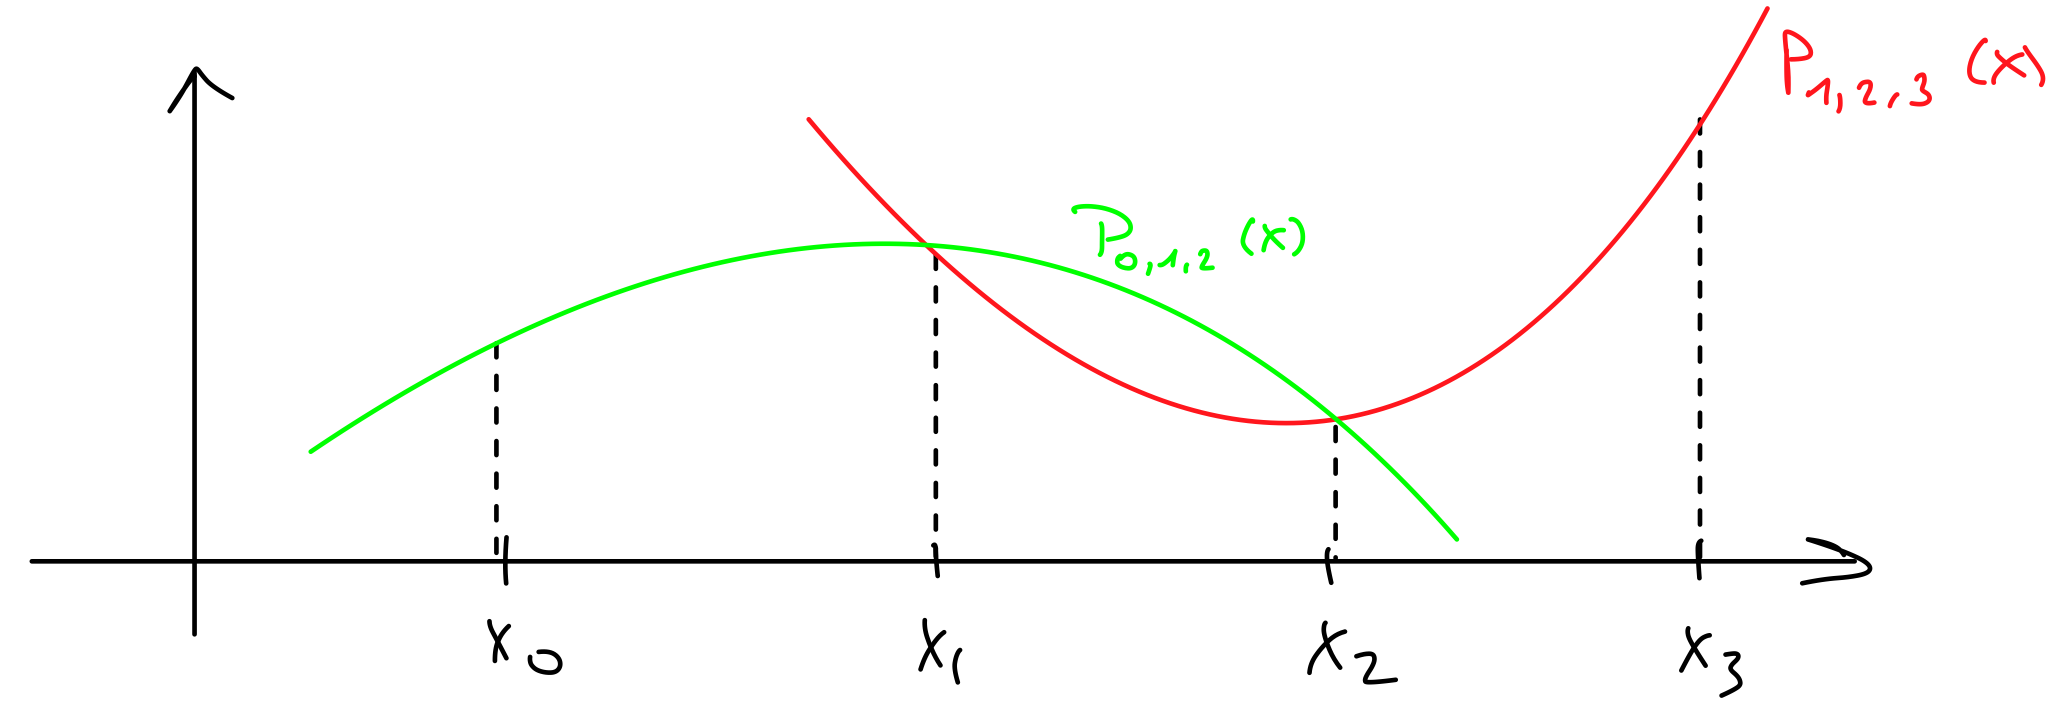
\includegraphics[width=0.5\linewidth]{img/neville.png}
\end{figure}
Here, 
\begin{equation}
    P_{0123}(x) = \frac{x-x_0}{x_3-x_0}\color{red}P_{123}(x)\color{black}+\frac{x_3-x}{x_3-x_0}\color{green}P_{012}(x)\color{black}
\end{equation}
\section{Newton's interpolation formula}
Newton's interpolation formula is used to evaluate polynomials with a computer, as it only needs to compute each operation \((x-x_i)\) one time. We write it like:
\begin{equation}
    p_n(x) = \left(\left(\dots\left(y_{0\dots n}(x-x_n)+y_{0\dots n-1}\right)(x-x_{n-1})+y_{0\dots n-2}\right)(x-x_{n-2})+\dots\right) + y_0
\end{equation}
And the recursive formula is
\begin{equation}
    P_{i_0i_1\dots i_k}= P_{i_0i_1\dots i_{k-1}}(x) + y_{i_0i_1\dots i_k}(x-x_{i_0})(x-x_{i_1})\dots(x-x_{i_{k-1}})
\end{equation}
\end{document}